\section{Metody przenoszenia obiektów do 3D}
Odkąd zaczęto wykorzystywać komputerową grafikę trójwymiarową do tworzenia
wirtualnych rzeczywistości zaszła potrzeba wynalezienia sposobu tworzenia jak
najprostszego i zarazem najlepszego sposobu odwzorowywania istniejących
przedmiotów w świecie wirtualnym. Ten rozdział przedstawia opis metodologii oraz
ogólny zarys wykorzystywanych aktualnie algorytmów służących do spełnienia
przedstawionego wymagania.

\subsection{Modelowanie obiektów}
Modelowanie obiektów jest jednym ze sposobów, które wymagają najwięcej
kreatywnej pracy. Modelowanie można zdefiniować jako proces tworzenia
trójwymiarowych obiektów przy użyciu specjalistycznego oprogramowania.
Trójwymiarowy obiekt jest zdefiniowany przy użyciu obiektów matematycznych
takich jak punkt, trójkąty, krzywe, powierzchnie. Na rynku istnieje wiele programów,
których funkcjonalność jest wystarczająca do przygotowania pełnego,
realistycznego modelu. Do najbardziej popularnych można zaliczyć Autodesk
Maya~\footnote{\url{http://usa.autodesk.com/maya/}}, Autodesk 3ds
Max~\footnote{\url{http://usa.autodesk.com/3ds-max/}}, MAXON Cinema
4D~\footnote{\url{http://www.maxon.net/}}, NewTek Lightwave
3D~\footnote{\url{http://www.newtek.com/lightwave.html}}, Pixologic
ZBrush~\footnote{\url{http://www.pixologic.com/zbrush/}}, Luxology
Modo~\footnote{\url{http://www.luxology.com/modo/index.aspx}} bądź darmowy
Blender~\footnote{\url{http://www.blender.org/}}.

Co prawda nie ma ściśle określonych reguł co do etapów występujących w procesie
tworzenia modelu ale ogólnie można wyróżnić kilka logicznych etapów (na
przykładzie modelowania głowy):
\begin{enumerate}
  \item przygotowanie kilku obrazów odniesienia modelowanej głowy;
  \item wstępne wydzielenie linii charakterystycznych;
  \item wykorzystanie krzywych (lub wielokątów) do zamodelowania kształtu głowy;
  \item uszczegółowienie i dopasowanie modelu;
  \item dodanie szczegółów (uszy, usta itp.);
  \item teksturowanie (brak wpływu na geometrię).
\end{enumerate}

Jak widać proces tworzenia modelu tą techniką jest bardzo czasochłonny i wymaga
nie tylko zajęcia się właściwym modelowaniem, ale także przygotowaniem danych
niezbędnych do dokładnego odwzorowania. W procesie takim można oczywiście 
wykorzystać poprzednio utworzone modele i je modyfikować, jednak nadal wymaga to
dosyć sporej ingerencji w samą strukturę geometryczną modelu przy tworzeniu
każdego kolejnego modelu.
Zdecydowaną wadą jest to, że jakość efektów osiąganych tą metodą nie zawsze
jest wystarczająca, gdyż zależy ona w głównej mierze od umiejętności i
cierpliwości osoby tworzącej obiekt.

\addtocounter{footnote}{1}
{
\begin{figure}[h]
  \centering
  \subfloat[Obrazy odniesienia.]{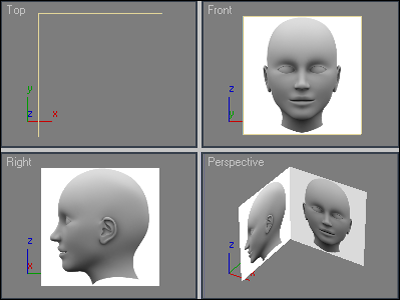
\includegraphics[width=6cm]{images/head_tut/1.png}}
  \quad
  \subfloat[Modelowanie warg.]{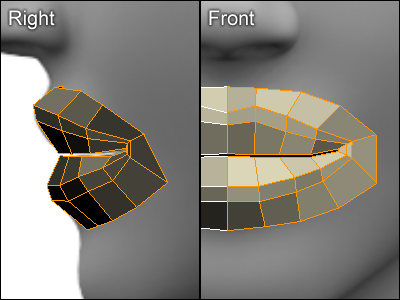
\includegraphics[width=6cm]{images/head_tut/4.png}}
  \label{mo_01}
  \caption[Modelowanie obiektów.]{Modelowanie obiektów~$^{\decimal{footnote}}$.}
\end{figure}
\begin{figure}[h]
  \centering
  \subfloat[Modelowanie policzków.]{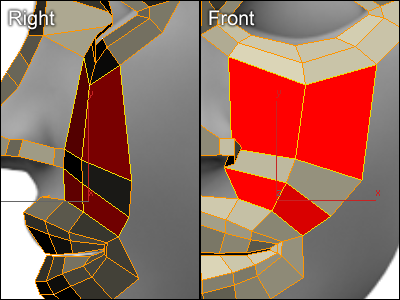
\includegraphics[width=6cm]{images/head_tut/6.png}}
  \quad
  \subfloat[Modelowanie nosa.]{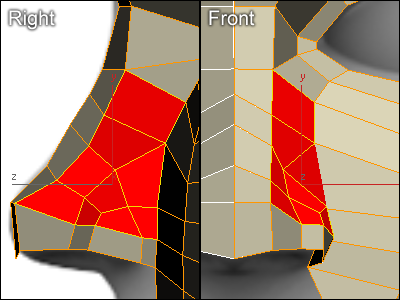
\includegraphics[width=6cm]{images/head_tut/7.png}}
  \label{mo_02}
  \caption[Modelowanie obiektów cd.]{Modelowanie obiektów~$^{\decimal{footnote}}$ cd.}
\end{figure}
\footnotetext[\value{footnote}]{Źródło:
\url{http://www.secondpicture.com/tutorials/3d/3d_modeling_of_a_human_head_3ds_max_01.html}} }

% !!!!!!! DORZUC JESZCZE TE OBRAZKI !!!!!!!!! po dwa w wierszu wystarczą 
%\begin{center}
%\begin{tabular}{c | c | c}
%  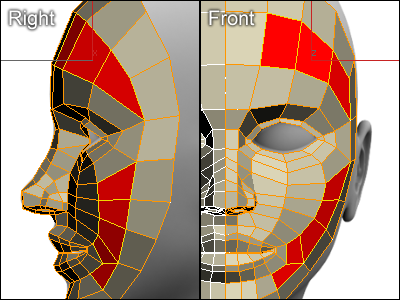
\includegraphics[width=4cm]{images/head_tut/9.png}
%  &
  %\caption{Wymodelowana twarz.}
%  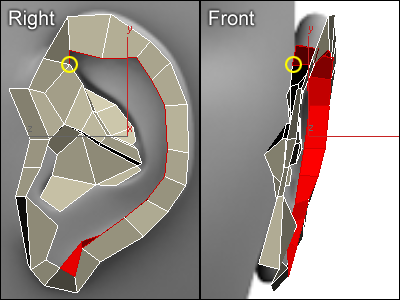
\includegraphics[width=4cm]{images/head_tut/11.png}
  %\caption{Modelowanie ucha.)&
%  &
 %\begin{figure}
%  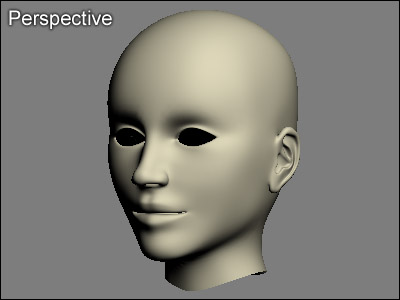
\includegraphics[width=4cm]{images/head_tut/12.png}
  %\caption{Finalny model po wygładzeniu.}
  %\end{figure}
%\end{tabular}
%\end{center}

\subsection{Modelowanie progresywne}
Jest to rozwinięcie zwykłego modelowania o wykorzystanie sekwencji obrazów
odniesienia zamiast pojedynczego tła. Proces tworzenia składa się z kilku
powtarzalnych kroków:
\begin{enumerate}
  \item oznaczenie nowych krawędzi obiektów;
  \item przejście do kolejnego ujęcia i ewentualne dodanie poprawek do
  naniesionych opisów krawędzi;
  \item powtórzenie kroków aż do uzyskania zadowalającego efektu.
\end{enumerate}

Niewątpliwą zaletą jest to, że podstawowy, nieskomplikowany model otrzymuje się
bardzo szybko. Model tworzy się poprzez generowanie siatki na obrazie
dwuwymiarowym, a dane przestrzenne są wyliczane automatycznie. Im więcej ujęć
jest dostępnych dla projektanta, tym lepsze efekty może osiągnąć. Z uwagi na to,
że algorytm bazuje na automatycznym wykrywaniu zmiany obrazu wymagane jest, aby
obrazy były dobrej jakości i w dobrym oświetleniu.
Kilka zrzutów ekranu z kolejnych kroków procesu tworzenia przykładowego modelu
zostało przedstawionych na ilustracjach \ref{progres1}, \ref{progres2},
\ref{progres3}, \ref{progres4}.

\addtocounter{footnote}{1}
\begin{figure}[h]
  \centering
  \subfloat[Modelowany obiekt]{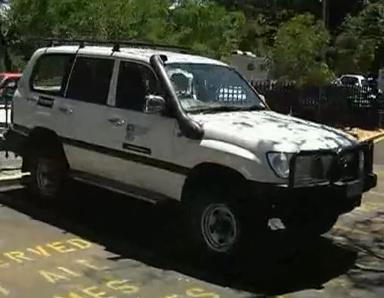
\includegraphics[width=6cm]{images/progr/1.png}\label{progres1}}
  \quad
  \subfloat[Początkowa struktura]{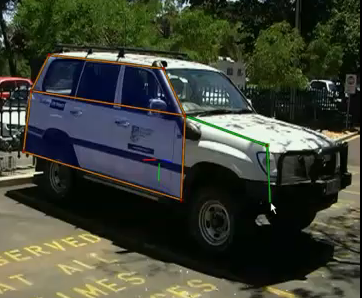
\includegraphics[width=6cm]{images/progr/2.png}\label{progres2}}
  \caption[Modelowanie progresywne.]{Modelowanie progresywne~$^{\decimal{footnote}}$.}
\end{figure}

\begin{figure}[h]
  \centering
  \subfloat[Struktura finalna]{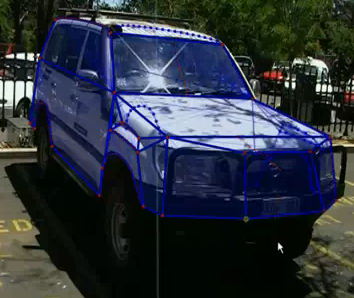
\includegraphics[width=6cm]{images/progr/3.png}\label{progres3}}
  \quad
  \subfloat[Wygenerowany obiekt]{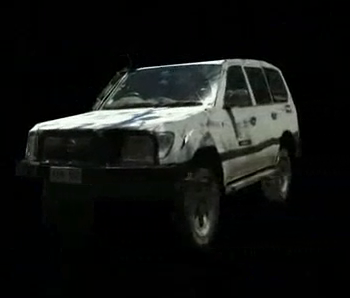
\includegraphics[width=6cm]{images/progr/4.png}\label{progres4}}
  \caption[Modelowanie progresywne cd.]{Modelowanie progresywne~$^{\decimal{footnote}}$cd.}
\end{figure}
\footnotetext[\value{footnote}]{Program
VideoTrace, \url{http://punchcard.com.au/wordpress/}}

\subsection{Modelowanie poprzez skanowanie}
Skanowanie jest to technika automatycznego tworzenia struktury oraz kolorów
trójwymiarowego modelu poprzez skanowanie powierzchni rzeczywistego modelu przy
użyciu specjalnych urządzeń. Urządzenia podczas skanowania tworzą chmurę
punktów, która później jest przetwarzana do dowolnego obsługiwanego formatu i
ewentualnie poddawana obróbce w programie modelującym. Technika skanowania jest
często używana, gdyż daje bardzo dokładne odwzorowanie obiektów. W zależności od
sposobu analizy struktury obiektu powstają pewne ograniczenia, jak np. problemy 
z powierzchniami, które charakteryzują się wysoką połyskliwością, problemy z
obiektami przeźroczystymi.

Skanery można podzielić na dwie grupy: odtwarzające kształt poprzez mechaniczny
kontakt oraz bezkontaktowe.

Skanery kontaktowe mają ograniczony zakres funkcjonalności z uwagi na to, że
wymagają fizycznego kontaktu z analizowanym obiektem, przez co obiekt może ulec
uszkodzeniu. Zaletą jest bardzo duża dokładność skanowania, natomiast wadą
jest powolność - z uwagi na mechaniczne przesuwanie sensora.

Skanery bezkontaktowe mają szerszy zakres używalności ponieważ nie niosą ze
sobą ryzyka uszkodzenia obiektu oraz, z uwagi na brak mechanicznego sensora,
mają o wiele większy zasięg i szybkość wykonywania skanowania. Ze względu na
sposób detekcji kształtu skanery tego typu dzielą się na aktywne i pasywne.
Skanery aktywne wysyłają jakiś typ promieniowania lub światła. Odległość do
obiektu może być wyliczana poprzez badanie czasu wędrówki wysłanych danych lub triangulując pozycje punktu lasera. Kształt może zostać
otrzymany również poprzez rzutowanie na obiekt ustalonego wzoru i jego ruch.
Detektor na podstawie zmiany rzutowanego wzoru względem oryginalnego odtwarza
kształt.
Skanery pasywne bazują na promieniowaniu istniejącym w środowisku (odbicie
światła, podczerwień) i nie emitują żadnych wiązek w kierunku obiektu. Do tej
grupy zaliczają się również skanery wyznaczające obrys z sekwencji obrazków,
gdzie obiekt jest umieszczony na tle o dużym kontraście.

\addtocounter{footnote}{1}
\begin{figure}[h]
  \centering
  \subfloat[Model
  1.]{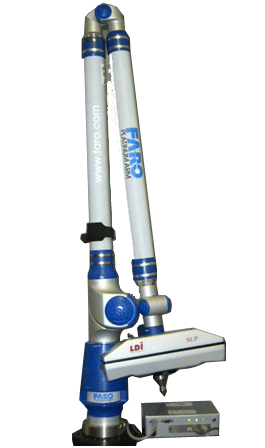
\includegraphics[width=4cm]{images/laser_scanner.png}\label{skan1}}
  \quad
  \subfloat[Model 2.]{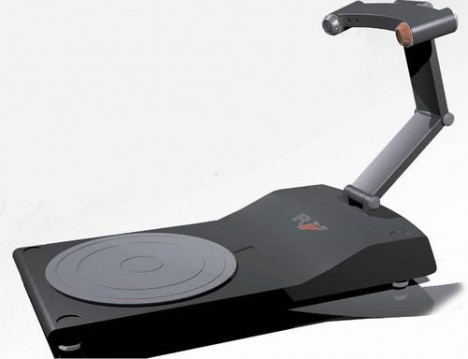
\includegraphics[width=6cm]{images/laser_scanner2.jpg}\label{skan2}}
  \caption[Lserowe skanery 3D]{Laserowe skanery 3D~$^{\decimal{footnote}}$.}
\end{figure}
\footnotetext[\value{footnote}]{Źródła:
\url{http://www.laserdesign.com/products/scanners_and_software/portable_laser_scanners/surveyor_fa-series/},
\url{http://www.coolest-gadgets.com/20090202/real-view-3d-scanner/}}

%\subsection{Modelowanie z wykorzystaniem wymiarowania}

%\subsection{Generowanie obiektów}
%\subsubsection{Modelowanie proceduralne}
%\subsubsection{Generowanie obiektu z wykorzystaniem gramatyki kształtu}
\subsection{Generowanie obiektu z wykorzystaniem gramatyki kształtu}
Tworzenie obiektów z użyciem gramatyk kształtu jest tematem dalszej części tej
pracy. Technika ta wykorzystuje opis struktury kształtu obiektu i relacji
pomiędzy jego elementami składowymi.